% !TEX TS-program = pdflatex
% !TEX encoding = UTF-8 Unicode

\documentclass[11pt]{article} % use larger type; default would be 10pt

\usepackage[utf8]{inputenc} % set input encoding (not needed with XeLaTeX)
\usepackage{csquotes}
\usepackage{alltt}
\usepackage{xcolor}
\usepackage{hyperref}
\usepackage{multirow}
\usepackage{float}
%\usepackage[francais]{babel}

%%% PAGE DIMENSIONS
\usepackage{geometry} % to change the page dimensions
\geometry{letterpaper} % or letterpaper (US) or a5paper or....
% \geometry{margins=2in} % for example, change the margins to 2 inches all round
% \geometry{landscape} % set up the page for landscape
%   read geometry.pdf for detailed page layout information

\usepackage{graphicx} % support the \includegraphics command and options
\graphicspath{ {image/} }

% \usepackage[parfill]{parskip} % Activate to begin paragraphs with an empty line rather than an indent

%%% PACKAGES
\usepackage{booktabs} % for much better looking tables
\usepackage{array} % for better arrays (eg matrices) in maths
\usepackage{paralist} % very flexible & customisable lists (eg. enumerate/itemize, etc.)
\usepackage{verbatim} % adds environment for commenting out blocks of text & for better verbatim
\usepackage{subfig} % make it possible to include more than one captioned figure/table in a single float
% These packages are all incorporated in the memoir class to one degree or another...

%%% HEADERS & FOOTERS
\usepackage{fancyhdr} % This should be set AFTER setting up the page geometry
\pagestyle{fancy} % options: empty , plain , fancy
\renewcommand{\headrulewidth}{0pt} % customise the layout...
\lhead{}\chead{}\rhead{}
\lfoot{}\cfoot{\thepage}\rfoot{}

%%% SECTION TITLE APPEARANCE
\usepackage{sectsty}
\allsectionsfont{\sffamily\mdseries\upshape} % (See the fntguide.pdf for font help)
% (This matches ConTeXt defaults)

%%% ToC (table of contents) APPEARANCE
\usepackage[nottoc,notlof,notlot]{tocbibind} % Put the bibliography in the ToC
\usepackage[titles,subfigure]{tocloft} % Alter the style of the Table of Contents
\renewcommand{\cftsecfont}{\rmfamily\mdseries\upshape}
\renewcommand{\cftsecpagefont}{\rmfamily\mdseries\upshape} % No bold!

%%%MACROS!
\newcommand{\system}[1]{\textsf{#1}}
\newcommand{\allo}{}
\newcommand{\JSB}{\system{JSrealB}}
\newcommand{\quo}[1]{"#1"}
\newcommand{\code}[1]{\texttt{#1}}
\newcommand{\real}[1]{\emph{#1}}
\floatstyle{ruled}
\newfloat{example}{h}{}
\floatname{example}{Exemple}
\newcommand*{\exampleautorefname}{Exemple}
\renewcommand{\tablename}{Tableau}
\renewcommand*{\tableautorefname}{Tableau}
\renewcommand*{\subsectionautorefname}{Sous-section}
\renewcommand*{\subsubsectionautorefname}{Sous-section}


\newcommand{\simpleExample}[2]{\begin{center}
                 \code{#1} \newline \real{#2}
                 \end{center}}


\newenvironment{tabExample}[2]
{\begin{tabular}{|p{8cm}|c|}
\hline
\begin{alltt}#1\end{alltt} & \real{#2} \\
\hline}
{\end{tabular}}

\newcommand{\abc}[2]{
\begin{}
  
  
\end{env}
}



%%% END Article customizations

%%% The "real" document content comes below...

\title{\JSB{}, un réalisateur de texte multilingue: maintenant à jour en
français et en anglais}
\author{Francis Gauthier\\Département d'Informatique et de Recherche Opérationnelle\\Université de Montréal}

\begin{document}
\maketitle

%%RÉSUMÉ

\begin{verse}
Sous la direction de Guy Lapalme, professeur au département d'informatique
et de recherche opérationnelle de l'Université de Montréal.
\end{verse}
\begin{description}
\item [{Résumé:}] Ce document est un rapport de stage écrit par Francis
Gauthier au sujet de son stage d'été au laboratoire RALI de l'Université
de Montréal, sous la tutelle de Guy Lapalme. Francis a travaillé sur
la reprise du projet \JSB{} qui avait été auparavant commencé par
deux autres étudiants du RALI. Le but du stage était de peaufiner
le programme et de lui ajouter plusieurs fonctionnalités qui n'avaient
pas été implémentées encore. 
\end{description}


%%TABLE DES MATIÈRES

\pagebreak
\begin{verse}
\tableofcontents{}
\end{verse}
\pagebreak

%%DÉBUT

\section{Introduction}

Au fil de son développement, \JSB{} a connu plusieurs étapes. En
2014, Nicolas Daoust a commencé le projet en créant \system{JSreal}. Il développa
un réalisateur de texte facilement adaptable au web en langage JavaScript.
Cette version n'était que francophone. L'année suivante, Paul Molins
a repris le projet et en a fait une version bilingue, en français
et en anglais. À l'aide d'une utilisation systématique de table de
règle et de lexiques annexes au programme, \system{JSreal} devint \JSB{}.
Le réalisateur de texte devint alors bilingue et prêt à accueillir
d'autres langues semblables au français et à l'anglais. Après 2015
et après les modifications de Paul, le projet est laissé sur la glace
avec plusieurs options à rajouter au programme. Entre autres, plusieurs
déclinaisons de phrase telles que les phrases interrogatives et négatives
n'étaient pas implémentées, dans les deux langues. L'élision avait
besoin d'être revue et les verbes aux temps composés n'étaient pas
pris en charge, entre autres. Francis Gauthier a donc repris le projet
à l'été 2016. Ce rapport fait état des modifications qu'il a apportées
à \JSB{}.

\section{Qu'est-ce que \JSB{}?}

La présente section présente le prototype de \JSB{} tel qu'il
était jusqu'en mai 2015 et le fonctionnement général du programme. 
Dans les sections suivantes(de 3 à 7) sont décrits
les changements apportés au prototype.

\JSB{} est un réalisateur de texte réalisant des phrases en français
et en anglais. La fonction première du programme est de prendre en
entrée une structure de données composés d'objets JavaScript
qui représente une structure d'arbre syntaxique.
\JSB{} donnera en sortie la phrase correspondante à l'arbre donné
en entrée. Parmi les parties complexes de la réalisation, on retrouve
les accords en genre et en nombre entre les différents constituants
de la phrase, l'application des différentes options prescrites par
l'utilisateur, ainsi que la mise en forme de la phrase. 

\subsection{Les objets \JSB{}}

L'\autoref{num1} démontrent des appels à \JSB{} et leur réalisations. À noter que
\JSB{} utilise une représentation de la structure d'une phrase en terme
de ses constituants syntaxiques.\newline
\begin{example}
\caption{Quelques utilisations}
\begin{tabular}{p{7cm} p{7cm}}
\begin{alltt}
S(NP(D('le'),
     N('chat')),
  VP(V('aimer'),
     NP(D('le'),
        N('jouet'))))
\end{alltt} &
\begin{alltt}
S(NP(D('le'),
     N('souris')),
  VP(V('partir').t("f"),
     PP(P("avant"),
        NP(D('le'),
           N('chat').n("p")))))
\end{alltt} \\
\real{Le chat aime le jouet.} & \real{La souris partira avant les chats.} \\
\end{tabular}
\label{num1}
\end{example}

Les appels en majuscule représentent des fonctions qui créent des objets \JSB{}. Ceux-ci sont
classés en deux catégories. 

\paragraph{Syntagmes}

Les syntagmes sont des groupes d'éléments de la phrase. Ceux-ci sont
des éléments passifs qui ne peuvent qu'exister s'ils ont des enfants.
Ils sont essentiels à la réalisation, car ils fournissent l'information
nécessaire pour comprendre les interactions entre les différents constituants
de la phrase. Si on pense à un arbre syntaxique, ces syntagmes représentent
les noeuds internes de l'arbre. La \autoref{tab:syntagmeTable} liste les syntagmes disponibles.
\begin{table}[h]
\centering
\caption{Les syntagmes}
\begin{tabular}{|l|l|l|}
\hline 
\multicolumn{1}{|c}{Appel \JSB{}}  & \multicolumn{1}{|c}{Syntagme} & \multicolumn{1}{|c|}{Exemple}\tabularnewline
\hline 
\hline 
\texttt{S} & Phrase & \real{Le chat aime le jouet}.\tabularnewline
\hline 
\texttt{NP} & Syntagme nominal & \real{le chat}\tabularnewline
\hline 
\texttt{VP} & Syntagme verbal & \real{aime le jouet}\tabularnewline
\hline 
\texttt{AP} & Syntagme adjectival & \real{très beau}\tabularnewline
\hline 
\texttt{AdvP} & Syntagme adverbial & \real{bien heureusement}\tabularnewline
\hline 
\texttt{PP} & Syntagme prépositionnele & \real{à la maison}\tabularnewline
\hline 
\texttt{CP} & Syntagme coordonné & \real{la pomme, la poire et la pêche}\tabularnewline
\hline 
\end{tabular}

\label{tab:syntagmeTable}
\end{table}


\paragraph{Éléments terminaux}

Les éléments terminaux font partie des syntagmes. Ils peuvent être
appelés sans syntagme, auquel cas leur réalisation sera simplifiée.
Chaque mot de la phrase est un élément terminal et ils sont classés
en fonction de leur classe de mots, selon les lexiques inclus dans le
programme. La \autoref{tab:terminauxTable} liste les éléments disponibles.

\begin{table}[h]
\centering
\caption{Les éléments terminaux}
\label{tab:terminauxTable}
\begin{tabular}{|l|l|l|}
\hline 
\multicolumn{1}{|c}{Appel \JSB{}}  & \multicolumn{1}{|c}{Classe de mot} & \multicolumn{1}{|c|}{Exemple}\tabularnewline
\hline 
\hline 
\texttt{V} & Verbe & \real{aimer}\tabularnewline
\hline 
\texttt{N} & Nom & \real{chat}\tabularnewline
\hline 
\texttt{D} & Déterminant & \real{le}\tabularnewline
\hline 
\texttt{A} & Adjectif & \real{beau}\tabularnewline
\hline 
\texttt{Pro} & Pronom & \real{je}\tabularnewline
\hline 
\texttt{P} & Préposition & \real{de}\tabularnewline
\hline 
\texttt{Adv} & Adverbe & \real{très}\tabularnewline
\hline 
\texttt{C} & Conjonction & \real{et}\tabularnewline
\hline 
\end{tabular}
\end{table}

\pagebreak{}
\subsection{Les transformations}

Chaque syntagme et élément terminal est un objet JavaScript, ce qui
lui permet d'avoir des propriétés propres. Ces propriétés sont principalement:
\begin{itemize}
\item[-] Le genre
\item[-] Le nombre
\item[-] La personne
\item[-] Le temps
\end{itemize}
Certains éléments recevront des propriétés par défaut du programme
lors de l'exécution. C'est-à-dire qu'un nom aura comme genre par défaut
le masculin et le nombre singulier. Un verbe recevra comme temps par
défaut l'infinitif. Outre la valeur par défaut, il est aisé pour
l'utilisateur d'en sprécifier d'autres. Les méthodes spécifiant les
propriétés voulues sont appelées directement sur les éléments terminaux
en question. La \autoref{tab:transfoTable} liste les principales transformations
disponibles.

\begin{table}[h]
\centering
\caption{Les transformations principales}
\label{tab:transfoTable}
\begin{tabular}{|l|l|l|l|}
\hline 
Propriété & Appel \JSB{} & Exemple d'appel & Réalisation\tabularnewline
\hline 
\hline 
Genre & g & \texttt{N("absent").g("f")} & \real{absente}\tabularnewline
\hline 
Nombre & n & \texttt{N("jeu").n("p")} & \real{jeux}\tabularnewline
\hline 
Personne & pe & \texttt{Pro("je").pe(2)} & \real{tu}\tabularnewline
\hline 
Temps & t & \texttt{V("aimer").t("i")} & \real{aimait}\tabularnewline
\hline 
\end{tabular}
\end{table}


Pour réaliser les différentes déclinaisons, le programme se base sur
deux fichiers JSON préalablement généré automatiquement à partir du 
lexique exhaustif \emph{dmf-lex}. 
\begin{itemize}
\item Le premier
est un \textbf{lexique} contenant les mots disponibles et le sigle de la table
de déclinaison correspondante au mot. 
\item Le deuxième regroupe les \textbf{tables
de règles} décrivant les différentes déclinaisons en genre et en nombre
de chaque sigle, ou les conjugaisons en fonction des temps et des
personnes pour les verbes.
\end{itemize}

Les syntagmes aussi peuvent subir des transformations. Par exemple,
si on désire modifier le genre de tous les éléments d'un syntagme,
il est possible de le spécifier sur le syntagme en tant que tel et
le programme propagera ces propriétés sur ses constituants enfants
durant l'exécution. Nous aborderons justement la propagation dans
la section suivante.

\subsection{La propagation}

Une des parties les plus importantes du programme est la propagation,
qui permet de réaliser les règles d'accords entre les différents constituants.
La propagation est le fait que certains constituants de la phrase
auront des propriétés dictées par l'utilisateur ou par défaut et que
ces propriétés doivent être partagées avec d'autres constituants de
la phrase pour faire en sorte de bien accorder les différentes sections
de la phrase. On note trois types de propagations différentes:

\paragraph{Propagation parent$\rightarrow$enfant}

Lorsqu'une propriété est attribuée à un syntagme, on croit que l'utilisateur
désire que cette propriété soit partagée entre tous ses constituants.
Donc, pour chacun des enfants d'un syntagme parent, ils recevront
les propriétés de leur parent immédiat.

\paragraph{Propagation frère/soeur}

À l'intérieur même d'un syntagme, on retrouve des éléments qui forment
le noyau ou des éléments subordonnés au noyau. Dans ce cas, les propriétés
du noyau seront propagées vers les éléments subordonnés pour que les
éléments formés dans le syntagme soient tous accordés de la même façon.
C'est cette propagation qui passera les informations du syntagme nominal
sujet au syntagme verbal principal pour l'accord du verbe, par exemple. 

\paragraph{Propagation enfant$\rightarrow$parent}

Certains noyaux nécessitent de transmettre leurs informations à leur
parent pour que ceux-ci transmettent ensuite l'information ailleurs.
C'est le cas pour le noyau du syntagme nominal(le nom) qui transmettra
ses propriétés à son parent.

À noter que la propagation arrive en second plan face aux propriétés
dictées par l'utilisateur. C'est-à-dire que les éléments possèdent
en général des propriétés par défaut, qui peuvent être supplantées
par les propriétés imposées par l'utilisateur. Ensuite, la propagation
peut changer les valeurs par défaut, mais ne pourra pas changer une
valeur imposée. La \autoref{fig:propag} démontre un peu l'effet de la propagation
sur les éléments et leurs réalisations.
\begin{figure}
\centering
\caption{La propagation}
\label{fig:propag}
%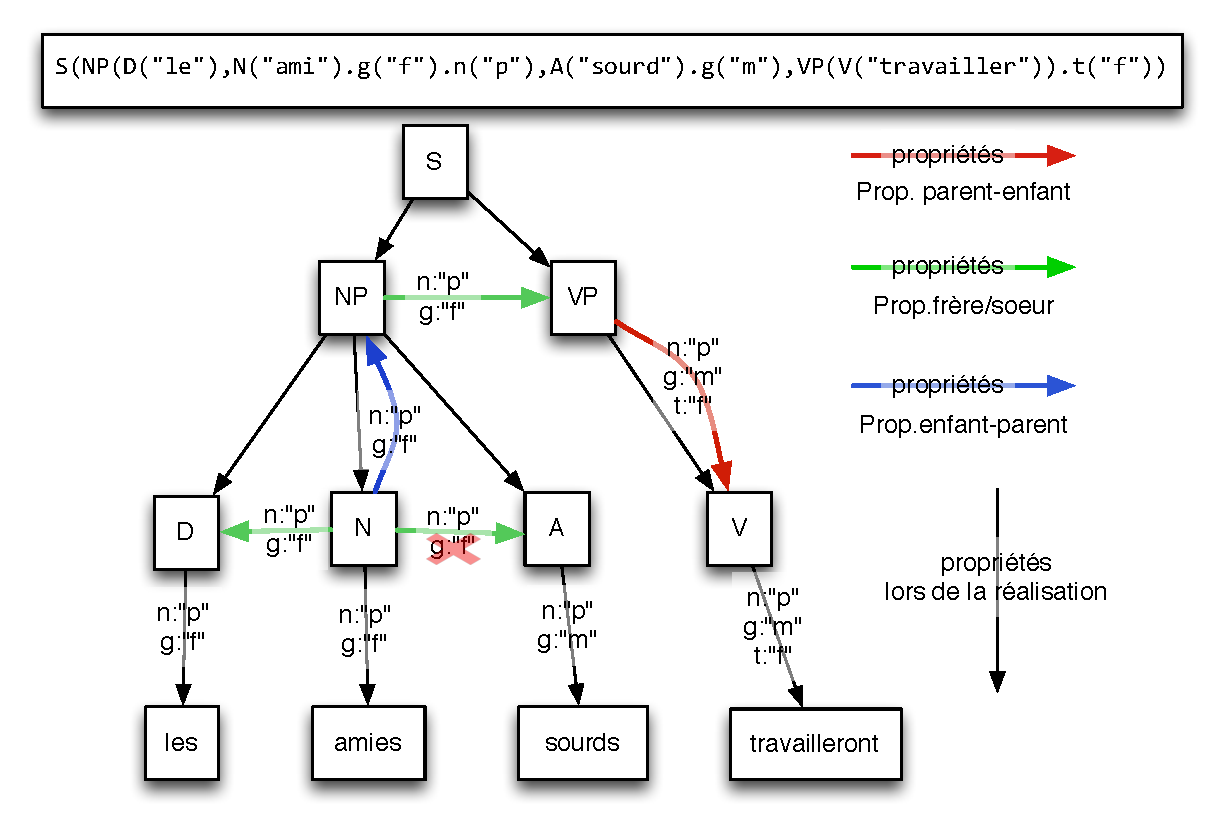
\includegraphics[scale=0.8]{Propagation}
\end{figure}

L'encadré du haut représente l'appel \JSB{}. Les éléments du bas sont ceux
réalisés. La phrase finale serait: \real{*Les amies sourds travailleront.}
On voit dans le schéma les trois types de propagations, représenté
par les flèches de couleurs. Il est intéressant de noter que la propagation
du genre du nom vers l'adjectif n'aura pas lieu, car dans l'appel
\JSB{}, l'utilisateur a spécifié que le genre de l'adjectif devait
être masculin. Cette spécification de l'utilisateur a priorité sur
la propagation.

À noter que dans la majorité des cas, l'utilisateur ne spécifiera pas
que quelques propriétés et que celles-ci seront propagées automatiquement
et de manière à respecter les règles de la langue choisie. C'est-à-dire qu'un
adjectif sera 00toujours bien accordé avec le nom auquel il est rattaché, à moins
que l'utilisateur désire autrement.

\subsection{Autres fonctionnalités}

\JSB{} a quelques autres fonctionnalités. Il s'occupe notamment de
la mise en forme des phrases. Il est possible de contrôler la mise
en majuscule au début des mots, de rajouter de la ponctuation additionnelle
et le programme comprend deux modules complémentaires très utiles,
soit \emph{Date} et \emph{Number}. Ces deux modules permettent l'intégration
des dates plus facilement à l'intérieur même des phrases, ainsi que
pour les nombres. 

Aussi, \JSB{} permet l'intégration des balises HTML, donc son intégration
est aisée sur le web. \\
\begin{example}
\caption{Utilisation d'un tag HTML}
\begin{alltt}
  N('joueur').tag('u')    \textnormal{(Appel)}
    
  <u>joueur</u>           \textnormal{(Réalisation \JSB{})}
\end{alltt}
\begin{tabular}{p{0.4cm} p{3.8cm} c}
 & \real{\underline{joueur}} & (Sur une page HTML)
\end{tabular}
\end{example}

\subsection{Exécution}
\label{subsec:exec}

Il est intéressant de comprendre le fonctionnement de \JSB{} et quelles
sont les étapes principales de l'appel à la réalisation finale.

Voici brièvement les étapes suivies pour chaque noeud interne(syntagme).
Comme la structure \JSB{} peut être représentée comme un arbre, les
étapes qui seront décrites sont appelées de manière récursive sur les
enfants de chaque noeud. La réalisation de l'arbre se fait par un
passage en profondeur (enfant d'abord). Les étapes en question sont:
\begin{enumerate}
\item Classer ses différents constituants (modificateur, noyau, subordonnée
ou complément)
\item Créer une liste ordonnée de ces constituants à réaliser
\item Réaliser chacun de ces constituants dans l'ordre prédéfini précédemment
\item Concaténer chaque réalisation pour former sa propre réalisation
\item Appliquer des règles de phonétique et de ponctuation sur sa réalisation
\end{enumerate}

\subsection{\system{SimpleNLG-EnFr}}

Il existe un réalisateur de texte anglais et français précurseur à
\JSB{}. SimpleNLG-EnFr est une adaptation de \system{SimpleNLG} faite par Pierre-Luc
Vaudry au cours de ses études au RALI du département d'informatique
de l'Université de Montréal. Le réalisateur \system{SimpleNLG} est capable
de générer un éventail plus grand que \JSB{}. Son implémentation
a été faite en Java. À la fin du projet de \JSB{}, on espérait que
les deux réalisateurs soient de même calibre. À cette fin, plusieurs
des fonctionnalités de \system{SimpleNLG-EnFr} qui n'existaient pas dans \JSB{}
ont été travaillées. Le travail de Pierre-Luc Vaudry a servi de modèle
pour orienter les modifications apportées à \JSB{}.

\section{Modifications apportées aux syntagmes}
Après le développement de \JSB{} jusqu'en 2015, la structure du programme
était bien implantée, mais plusieurs fonctionnalités étaient manquantes.
Vous trouverez dans la section suivante quelques modifications qui
ont été faites au niveau des syntagmes.

Lors d'ajout aux possibilités de \JSB{}, il était évident
que certaines fonctionnalités allaient demander des ajouts mineurs,
alors que plusieurs autres nouvelles fonctions du réalisateur de texte nécessiteraient
de déconstruire certaines sections de l'arbre syntaxique et possiblement
de rajouter des éléments à cet arbre. Quatre options principales ont
demandé à réarranger la structure de l'arbre syntaxique en cours d'exécution:
la \textbf{phrase passive}, la \textbf{pronominalisation} d'un syntagme
nominal, la \textbf{phrase impérative} et la \textbf{phrase interrogative}.


Par exemple, pour la phrase impérative, il faut s'assurer de retirer
le sujet, si l'utilisateur ne l'a pas fait lui-même. Les différentes
étapes citées à la \autoref{subsec:exec} seront interrompues dans le fil d'exécution
après l'étape 3 pour réajuster la structure de l'arbre. Ensuite, on
retournera à la racine de l'arbre pour recommencer la réalisation
de départ. Cette étape est nécessaire, car, dans la phrase passive,
le sujet et le complément d'objet direct sont inversés et il est utile
de laisser \JSB{} refaire la propagation du nouveau sujet du nouvel
arbre pour éviter les conflits qui pourraient résulter d'une modification
manuelle. Il est donc important de comprendre que pour une phrase
avec peu d'options, soit une phrase assez simple, l'arbre sera traversé
en profondeur pour accomplir la réalisation, mais que si les options
précédentes sont présentes, la réalisation d'un arbre peut nécessiter
plusieurs passages de l'arbre. Même une phrase assez complexe
ne prendra que peu de passages, car les options sont assez limitées
et certaines options sont incompatibles avec d'autres, notamment la
phrase impérative, interrogative ou passive, qui sont incompatibles
entre elles.

\subsection{Syntagme nominal}

\subsubsection{Pronominalisation}
\label{pronomi}

La principale modification apportée à \JSB{} dans le syntagme nominal
est la possibilité de le pronominaliser. Par la pronominalisation,
on veut faire l'action de prendre un groupe nominal et le transformer
en un pronom. Par exemple, \emph{le garçon $\rightarrow$ il}. La
pronominalisation se fait essentiellement par la création d'un nouvel
objet de type \emph{pronom} qui héritera des propriétés qu'avait anciennement
le syntagme nominal. Le positionnement de ce nouvel objet
dans l'arbre syntaxique dépend de sa fonction dans la phrase. Si le syntagme
original avait une fonction de
\begin{itemize}
\item \textbf{sujet} dans la phrase, il sera remplacé par un pronom 
personnel; \emph{je }ou \emph{I}, décliné à la bonne personne.
\item \textbf{complément d'objet indirect}, on le remplace par un pronom
personnel; \emph{moi }ou \emph{me, }décliné à la bonne personne.
\item \textbf{complément d'objet
direct}, on remplace le syntagme par le pronom \emph{me}, en anglais. En français,
ce sera le pronom \emph{le}, tous deux déclinés selon la personne voulue.
\end{itemize}
Dans les deux premiers cas et dans le cas du complément d'objet direct \textbf{anglais},
les pronoms prennent la place du nom qu'ils remplacent.

Par contre, pour le complément d'objet direct \textbf{français}, c'est un peu plus complexe.
On doit changer pour le pronom \emph{le}
décliné selon la personne, mais on doit placer le pronom \textbf{avant} le
verbe. \JSB{} devra donc modifier les éléments du syntagme verbal
associé pour y changer la position du complément d'objet direct. Ce
faisant, le complément d'objet direct se déplace avant le verbe et
peut causer l'accord d'un participe passé employé avec \emph{avoir.
}La modification à la structure demandera de recommencer la réalisation
de l'arbre initial pour le nouveau.

La pronominalisation
du sujet fonctionne très bien, par contre on observe
des problèmes pour l'objet indirect. Les phrases obtenues sont
syntaxiquement correctes, mais diffèrent un peu du résultat attendu.
Par exemple, en pronominalisant l'objet indirect de cette phrase:
\emph{allons à la maison} ou \emph{go to the house, }on obtiendra
\emph{allons à elle }et \emph{go to him}. 

On s'attendrait à un pronom\emph{
}neutre en anglais comme \emph{it}(\emph{go to \textbf{it}}), mais le genre par défaut est toujours
masculin. Le changement vers un genre par défaut neutre offrirait certains avantages, 
notamment une meilleure pronominalisation, mais viendrait encombrer l'utilisateur
qui voudrait appeler un pronom simple comme sujet. L'appel de \texttt{Pro("I")}, renvoie 
actuellement \emph{he}, alors qu'avec le genre neutre par défaut, on obtiendrait \emph{it},
ce qui n'est pas désiré, étant donné que le sujet est plus souvent une personne qu'un objet.

En français, on pourrait préférer \emph{allons-y ou allons
là-bas} à la place de \emph{allons à elle}. L'utilisation de \emph{là-bas} demanderait une connaissance sémantique,
soit de savoir qu'on parle d'un lieu et l'utilisation du pronom \emph{y}
est restreinte à certaines prépositions du complément d'objet indirect.
Ces cas sont rares et n'amélioraient que peu le programme par rapport à la difficulté
engendrée pour repérer ces cas. 

Pour ce qui est de la pronominalisation du \textbf{complément d'objet
direct}, cela fonctionne assez bien, sauf lorsque d'autres options viennent
modifier la structure de la phrase. Par exemple, la pronominalisation du complément
d'objet direct avec un verbe négatif n'est pas encore pris en compte:\\
\begin{example}
\centering
\caption{La pronominalisation et le négatif, simultané}
\begin{tabular}{p{8cm} p{8cm}}
\begin{alltt}
S(Pro("je").pe(1),
  VP(V("voir").vOpt(\{neg:true\}),
     NP(D("mon").pe(2),
        N("lunette").n("p"))))
\end{alltt} &
\begin{alltt}
S(Pro("je").pe(1),
  VP(V("voir").vOpt(\{neg:true\}),
     NP(D("mon").pe(2),
        N("lunette").n("p")).pro()))
\end{alltt} \\
\real{Je ne vois pas tes lunettes.} & \real{*Je les ne vois pas.}
\end{tabular}
\end{example}

\subsection{Syntagme verbal}

\subsubsection{Temps composés}

Au moment de sa reprise, \JSB{} était en mesure de conjuguer les
verbes à leurs formes simples.Nous avons ajouté la conjugaison des temps composés.
Cela impliquait d'ajouter un ou plusieurs auxiliaires et un participe qui devra
aussi s'accorder en français.

\paragraph{Commun aux deux langues}

Dans les deux langues, on retrouve des auxiliaires, principalement 
\emph{avoir} et \emph{être}. Les deux langues ont des participes: 
présent et passé. Chaque verbe présent dans le lexique est 
lié à une table de règles qui 
permet de conjuguer les temps simples facilement. D'ailleurs, l'accord 
du participe passé ou présent est indiqué dans les tables. Ces fonctionnalités 
seront exploitées pour réaliser les temps composés, mais de manière assez 
différente entre les deux langues.

\paragraph{Français}

Le français contient huit temps simples, formés d'un seul verbe accordé fourni
dans les tables de règles. Ceux-ci sont:
\begin{itemize}
\item[-] Présent de l'indicatif
\item[-] Imparfait
\item[-] Impératif présent
\item[-] Futur simple
\item[-] Passé simple
\item[-] Conditionnel présent
\item[-] Subjonctif présent
\item[-] Subjonctif imparfait
\end{itemize}
Seuls les temps subjonctifs requierent le préfixe \emph{que}, 
mais autrement, ils se ressemblent tous dans leur manière de s'accorder. Il n'y 
a que deux auxiliaires possibles en français, soit \emph{avoir} et \emph{être}.
Ces auxiliaires dépendent du verbe à conjuguer.

La première étape de l'implémentation
a été l'ajout des auxiliaires au lexique qui ne comportait pas
d'information sur les auxiliaires. Ces informations
étaient disponibles dans les fichiers à partir desquels est généré
le lexique. Il a donc fallu quelques lignes de code pour extraire
cette information supplémentaire de nos ressources. À partir du moment
où le lexique a été actualisé avec ces modifications, on retrouvait
alors un attribut à chaque verbe dans le lexique. L'attribut \emph{aux
}du lexique a comme valeur possible \texttt{êt}:\emph{être}, \texttt{av}:\emph{avoir}
ou \texttt{aê}:\emph{être ou avoir}.

Les verbes qui comportaient
deux auxiliaires, par exemple le verbe \emph{changer,} sont accordés
avec l'auxiliaire \emph{avoir}. Moins de 3\% des verbes présents dans le
lexique ont cette propriété. Il est toutefois possible de forcer l'utilisation 
d'un auxiliaire autre que celui par défaut
avec l'option \texttt{.aux("être")} ou \texttt{.aux("avoir")} sur un verbe ou un syntagme verbal.

En bref, pour accorder un temps
composé, on appellera à nouveau la fonction de conjugaison, avec comme
paramètres:
\begin{itemize}
\item[-] l'auxiliaire tiré du lexique
\item[-] le temps de l'auxiliaire (tiré d'une table de règle)
\item[-] les éléments de propagation du verbe en question (personne, genre et nombre par exemple).
\end{itemize}
L'auxiliaire obtenu
sera ensuite concaténé avec le participe passé du verbe. Le participe passé 
en français requiert
parfois un accord, donc la fonction qui sera appelée ne sera pas celle
de conjugaison générale, mais une fonction particulière pour l'accord du
participe passé, qui sera décrite à la \autoref{subsec:accordpp}. Plusieurs
autres mots auxiliaires et adverbes peuvent se glisser entre ou autour
du verbe et de son auxiliaire. Ceux-ci sont décrits à la section
\autoref{subsec:vOptions}.

\paragraph{Anglais}

Les temps simples, c'est-à-dire ceux qui ne requièrent pas d'auxiliaire
sont le \emph{present tense} et le \emph{past tense}. Dans le module de
conjugaison, on intégrera le \emph{future tense} comme un temps simple, même si 
ce temps requiert l'utilisation de l'auxiliaire \emph{will}.
Il existe plusieurs verbes auxiliaires qui changent
le sens du verbe en anglais. Les deux principaux auxiliaires sont \emph{be}
et \emph{have}, mais on retrouve aussi \emph{will} et \emph{do} très souvent.

Une phrase complexe en anglais requiert l'utilisation de plusieurs verbes auxiliaires,
comme dans l'exemple \real{I will not have been going}. Dans l'exemple
précédent, \emph{will}, \emph{have} et \emph{been} sont tous des verbes
auxiliaires. En anglais,
les verbes auxiliaires dépendent \textbf{du temps de verbe} et non pas du 
verbe en tant que tel. Les temps composés sont les
temps \emph{perfect}, soit:
\begin{itemize}
\item[-]present perfect
\item[-]past perfect
\item[-]future perfect
\end{itemize} Ces temps requièrent tous d'appliquer l'auxiliaire
\emph{être} et le participe passé. Par contre, en ajoutant les options
de verbe, soit la forme passive, progressive(dite \emph{continuous}
en anglais), les auxiliaires changeront dépendamment de la combinaison
des options. Le fonctionnement sera détaillé à la \autoref{subsec:vOptions}.

\subsubsection{Accord du participe passé}
\label{subsec:accordpp}
En français, le participe passé doit s'accorder en fonction de son
auxiliaire. 

\paragraph{Accordé seul}

Comme dans le groupe nominal \emph{les fenêtres ouvertes.} Dans ce cas,
il faut propager les propriétés
de genre et de nombre aux verbes dans le syntagme
nominal. Ainsi, lors de l'appel de conjugaison du verbe
au participe passé, les propriétés du noyau nominal sont passées en
paramètre et un appel simple d'accord au participe passé réalisera
l'accord en genre et en nombre.

\paragraph{Accordé avec \emph{être}}

On s'assure d'abord que le verbe est dans une forme composée,
à l'instar du participe passé employé seul. Tout comme employé seul, le participe
recevra les informations du sujet pour s'accorder. Ensuite, comme le lexique
contient maintenant les informations sur les auxiliaires de chaque
verbe, il suffit de décliner le participe passé selon une table de
règle.

\paragraph{Accordé avec \emph{avoir}}

Il est très difficile d'accorder le participe, car il doit s'accorder en genre et en nombre avec
son complément d'objet direct, si celui-ci apparaît avant le verbe. Le
premier type de phrase où un tel accord est nécessaire est un syntagme
nominal à l'intérieur duquel on trouvera un syntagme propositionnel
complément au nom, par exemple: \emph{Les maisons que nous avons rencontrées.}
La première étape pour implémenter cet accord a été de mettre en place
le syntagme propositionnel, décrit à la \autoref{syntProp}.
Ensuite, les informations du noyau (\emph{maison}) sont propagées
vers les éléments du syntagme verbal en fonction du premier pronom
rencontré. C'est-à-dire que dans l'exemple plus haut, le pronom introduisant
la proposition est \emph{que,} et dans ce cas, la proposition aura
comme complément d'objet direct le syntagme nominal auquel il réfère \emph{(les
maisons}). Dans le cas où le syntagme propositionnel
est \emph{qui, }comme dans l'exemple \emph{Les garçons qui jouent
des tours,} alors le syntagme nominal \emph{les garçons }agit en tant
que sujet à la proposition. La propagation transmettra les informations de genre et de nombre
du sujet pour accorder le verbe en conséquence. Dans le cas où le premier pronom est \emph{que,
}les informations du complément d'objet direct sont passées en paramètres
au module de conjugaison qui accordera le participe passé avec auxiliaire
avoir, s'il y en a un.

Le deuxième type de phrase où le participe passé devait être accordé
avec avoir est une phrase où un pronom fait office de complément d'objet
direct placé avant le verbe, comme dans la phrase \emph{les pommes,
je les ai cueillies, }ou bien \emph{je l'ai appréciée, ta soeur. }En
prenant comme exemple la phrase \emph{les pommes, je les ai cueillies,
}il nous aurait fallu la structure suivante:
\begin{example}
\caption{Utilisation simple d'un pronom}
\begin{alltt}
S(NP(D("le"),
     N("pomme").n("p")),
  Pro("je").pe(1),
  VP(Pro("le").pe(3).n("p"),
     V("cueillir").t("pc")))
\end{alltt}
\real{*Les pommes, je les ai cueilli.}
\end{example}

Dans cette structure, le pronom \emph{les} est inclus manuellement.
Le lecteur sait que \emph{les} a comme antécédent \emph{les pommes},
mais pour un programme informatique, il n'existe pas de lien entre
les deux. 

Pour ne pas avoir à spécifier les antécédents, il est
plus pratique d'utiliser une pronominalisation des syntagmes
nominaux, discutée à la \autoref{pronomi}. Celle-ci est très utile pour
faire apparaître des pronoms avec les propriétés de leurs
antécédents, car ils ont été construits à partir de ceux-ci. Lors
de la pronominalisation, si le syntagme nominal est dans le syntagme
verbal, on considère qu'il est alors complément d'objet direct. En
le pronominalisant, le pronom vient se placer avant le verbe, ce qui
crée une situation où le participe passé devra s'accorder. C'est alors
que \JSB{} propagera les propriétés du pronom au verbe comme étant
celles de l'objet direct lui étant associé.

En combinant ces deux types de phrases, \JSB{} peut
accorder le participe passé avec l'auxiliaire avoir dans
la plupart des cas. Par contre, avec
des phrases plus complexes ou des figures de style, il probable que
la propagation ne se fasse pas correctement, surtout si l'accord du
participe passé requiert une interprétation humaine. Il
est d'ailleurs à noter que \JSB{} ne réalise en ce moment que des
phrases individuelles, donc si l'antécédent d'un pronom se trouve
dans une phrase différente, il ne serait possible de les accorder que
par le passage d'une variable globale. Voir la \autoref{clone}, pour plus de détails.


\subsubsection{Les verbes impératifs}
\label{imperatif}
L'utilisation du verbe à l'impératif était disponible dans la dernière
version de \JSB{}, mais peu complétée. Tout d'abord, un verbe appelé
sans option précisée par l'utilisateur recevra la troisième personne
du singulier comme valeur par défaut. Suite à une légère modification,
celle-ci a été changée pour la deuxième personne du singulier dans
le cas d'un appel à l'impératif pour éviter de générer des erreurs
fréquentes.

Par la suite, un retrait du groupe sujet a été ajouté au programme.
L'ajout a été fait dans l'optique d'un appel de l'impératif automatisé
sur une phrase qui contenait auparavant un sujet. Le retrait du sujet
de la structure de l'arbre syntaxique requiert de recommencer la réalisation
de l'arbre, car cela pourrait entrainer un accord du verbe différent.

\subsubsection{Les options}
\label{subsec:vOptions}
\paragraph{Commun aux deux langues}
Les quatre options suivantes ont été ajoutées à \JSB{}:
\begin{itemize}
\item la phrase négative
\item la phrase passive
\item la phrase progressive
\item le temps \emph{perfect}(en anglais)
\end{itemize} 
Comme ces options étaient fortement liées aux verbes, elles sont utilisées
comme des options directement sur les verbes. Voici un appel typique pour les options de verbe: 
\begin{example}
\caption{Utilisation des options de verbe}
\begin{alltt}
{V("manger").vOpt(\{pas:true,prog:false,neg:true\})}
\end{alltt}
\real{n'est pas mangé}
\end{example}

\paragraph{Français}

\subparagraph{Négation}

La négation se fait par l'ajout de deux adverbes en français. Le \emph{ne}
et le \emph{pas}, principalement. Il est possible d'avoir un
deuxième adverbe différent de \emph{pas}, c'est pourquoi il est possible
de préciser le second adverbe de négation en français dans \JSB{},
par contre, seule une liste restreinte d'adverbes sont acceptés, notamment
\emph{aucun, plus,rien, guère, etc... }En général, l'adverbe
\emph{ne }se place devant le verbe et l'adverbe \emph{pas,}après.
Par contre, lors de l'utilisation d'un temps composé, le deuxième
adverbe de négation se place entre l'auxiliaire et le participe passé.
C'est, entre autres, une des raisons pourquoi la négation est gérée
dans le module de conjugaison et non pas ailleurs. L'\autoref{negEx} démontre quelques
exemples de réalisations avec l'option négative:
\begin{example}
\caption{Utilisation de l'option négative}
\begin{alltt}
S(Pro("je"),
  VP(V("trouver").t("p").vOpt(\{neg:true\})))
\end{alltt}
\real{Il \textbf{ne} trouve \textbf{pas}.}\\

\begin{alltt}
S(Pro("je"),
  VP(V("trouver").t("pc").vOpt(\{neg:true\})))
\end{alltt}
\real{Il \textbf{n'}a \textbf{pas} trouvé.}\\

\begin{alltt}
S(Pro("je"),
  VP(V("trouver").t("pc").vOpt(\{neg:"rien"\})))
\end{alltt}
\real{Il \textbf{n'}a \textbf{rien} trouvé.}\\
\label{negEx}
\end{example}
\subparagraph{Passif}

La forme passive d'une phrase a demandé beaucoup plus de travail.
D'abord, le verbe doit être accordé différemment. Principalement,
les verbes avec l'auxiliaire \emph{avoir} s'accorderont désormais
avec l'auxiliaire \emph{être.} Si le syntagme nominal
a un sujet, alors le module de conjugaison rajoutera \emph{par}
à la fin du verbe.

La phrase devra également modifier sa
structure pour accommoder le mode passif. Le programme réagira au
fait que l'option passive a été déclarée en inversant le complément
d'objet direct du verbe avec le sujet. \\
\begin{example}
\caption{Utilisation de l'option passive}
\begin{tabular}{p{7cm} p{7cm}}
\begin{alltt}
S(NP(D("le"),
     N("chat"))
  VP(V("manger"),
     NP(D("le"),
        N("souris"))))
\end{alltt} &
\begin{alltt}
S(NP(D("le"),
     N("chat"))
  VP(V("manger").vOpt(\{pas:true\}),
     NP(D("le"),
        N("souris"))))
\end{alltt}
\\
\real{Le chat mange la souris.} & \real{La souris est mangée par le chat.}
\end{tabular}
\label{passif}
\end{example}
\\
Dans l'\autoref{passif}, dans la première phrase, \emph{le chat} était sujet, alors que dans la
deuxième phrase, il devient complément d'objet indirect. \emph{La souris}, quant à elle, 
est passée de complément d'objet direct à sujet de la phrase.

Il est possible que le sujet ou le complément d'objet direct ou les deux soient absents, auquel cas
il n'y aura qu'un déplacement d'une section de la phrase au lieu d'une
inversion. 

Étant donné que le sujet a possiblement changé suite à
cette inversion, il est essentiel de reprendre la propagation
pour que de nouveaux accords se fassent en fonction de la nouvelle
phrase. \JSB{} utilisera une fonction pour réinitialiser les propriétés
héritées des noeuds parents ou frères/soeurs de l'arbre. Ensuite,
la réalisation de l'arbre recommencera du début pour rétablir la bonne
propagation entre les nouveaux constituants de la phrase.

\subparagraph{Progressif}

La forme progressive spécifie que l'action est en cours, en ce moment même. 

Il suffit de rajouter le groupe de
mots \emph{en train de}. Dans le module de conjugaison, ce petit groupe de
mots est inséré habituellement entre l'auxiliaire et le participe
passé (s'il y en a un). Si le verbe n'est pas à un temps composé,
il faudra rajouter un auxiliaire \emph{être }pour obtenir la phrase
\emph{il est en train de manger}, par exemple. Il est aussi alors
nécessaire d'accorder le verbe participe à l'infinitif. Toutes ces
particularités sont gérées dans le module de conjugaison et peuvent
dépendre fortement des autres options de verbe pour occasionner des
cas légèrement différents.

\paragraph{Anglais}

\subparagraph{Négation}

Pour la négation, il n'y a qu'un adverbe de négation 
\emph{not. }L'adverbe de négation est habituellement placé entre un
premier verbe auxiliaire et le participe, comme dans \emph{I will
not love. }Pour les temps simples (present et past), il n'y a pas d'auxiliaire,
mais on doit rajouter l'auxiliaire \emph{do/did} dans ce cas. Par
exemple, \emph{I do not love you. }Finalement, le verbe \emph{to be},
représente une exception, au sens où il ne nécessite pas l'auxiliaire
\emph{do }aux temps simples. Dans ce cas précis, l'adverbe de négation
se place à la suite du verbe, comme dans \emph{I am not.} Cette exception
à la langue est une des rares exceptions que \JSB{} prend en compte,
car on s'attend à ce que son utilisation soit fréquente.

{*}À noter que la contraction de \emph{do not }vers \emph{don't} n'est
pas prise en charge, étant donné que la première forme est toujours
acceptée. Un ajout aux fonctions d'élision pourrait possiblement ajouter
cette option.
\subparagraph{Passif, progressif et parfait}

Les trois options s'influencent entre elles pour changer le
résultat de la réalisation du verbe. Lors d'un appel à la réalisation
d'un verbe avec des options, la réalisation se fera progressivement
par des appels récursifs aux fonctions de conjugaison du module de
conjugaison de \JSB{}. En anglais, le fonctionnement est différent
de celui en français qui passe plutôt par plusieurs tests, sans trop
de récursivité. Pour chaque option de verbe activée, le programme ajoutera
un auxiliaire et un participe dans les temps prescrits par la table
des règles qui fût ajoutée aux ressources de \JSB{}. Ceux-ci
sont listés dans le \autoref{tab:vOptionsEng}: 
\\
\begin{table}
\centering
\caption{Les options de verbe anglais et leur participes}
\begin{tabular}{|l|l|l|}
\hline 
Option de verbe & Auxiliaire & Participe\tabularnewline
\hline 
\hline 
passive (\texttt{pas)} & \emph{be} & passé\tabularnewline
\hline 
continuous (\texttt{prog)} & \emph{be} & présent\tabularnewline
\hline 
perfect (\texttt{perf)} & \emph{have} & passé\tabularnewline
\hline 
\end{tabular}
\label{tab:vOptionsEng}
\end{table}
\\
Pour que la réalisation se fasse, le programme vérifie, dans l'ordre
suivant: \emph{passif,progressif} puis \emph{perfect}, si une de ces options est
activée. Si l'option est activée, le résultat de la réalisation de
cette étape du verbe sera la concaténation du verbe auxiliaire au
temps prescrit pas l'appel initial du verbe(present, past ou future)
ainsi que de l'appel du verbe initial au participe passé/présent selon
la règle. Ensuite, l'option qui vient d'être utilisée sera désactivée et les options
de verbe résultantes seront passées en paramètres pour l'accord de
l'auxiliaire. Celui-ci pourrait encore avoir des options de verbe
à consommer, donc il devra refaire l'étape décrite récursivement,
mais avec une option de verbe différente. \autoref{figvOptEn} explique
 la réalisation du verbe \emph{to love}, avec les trois options
de verbe initialement activées.
\begin{figure}
\centering
\caption{}
%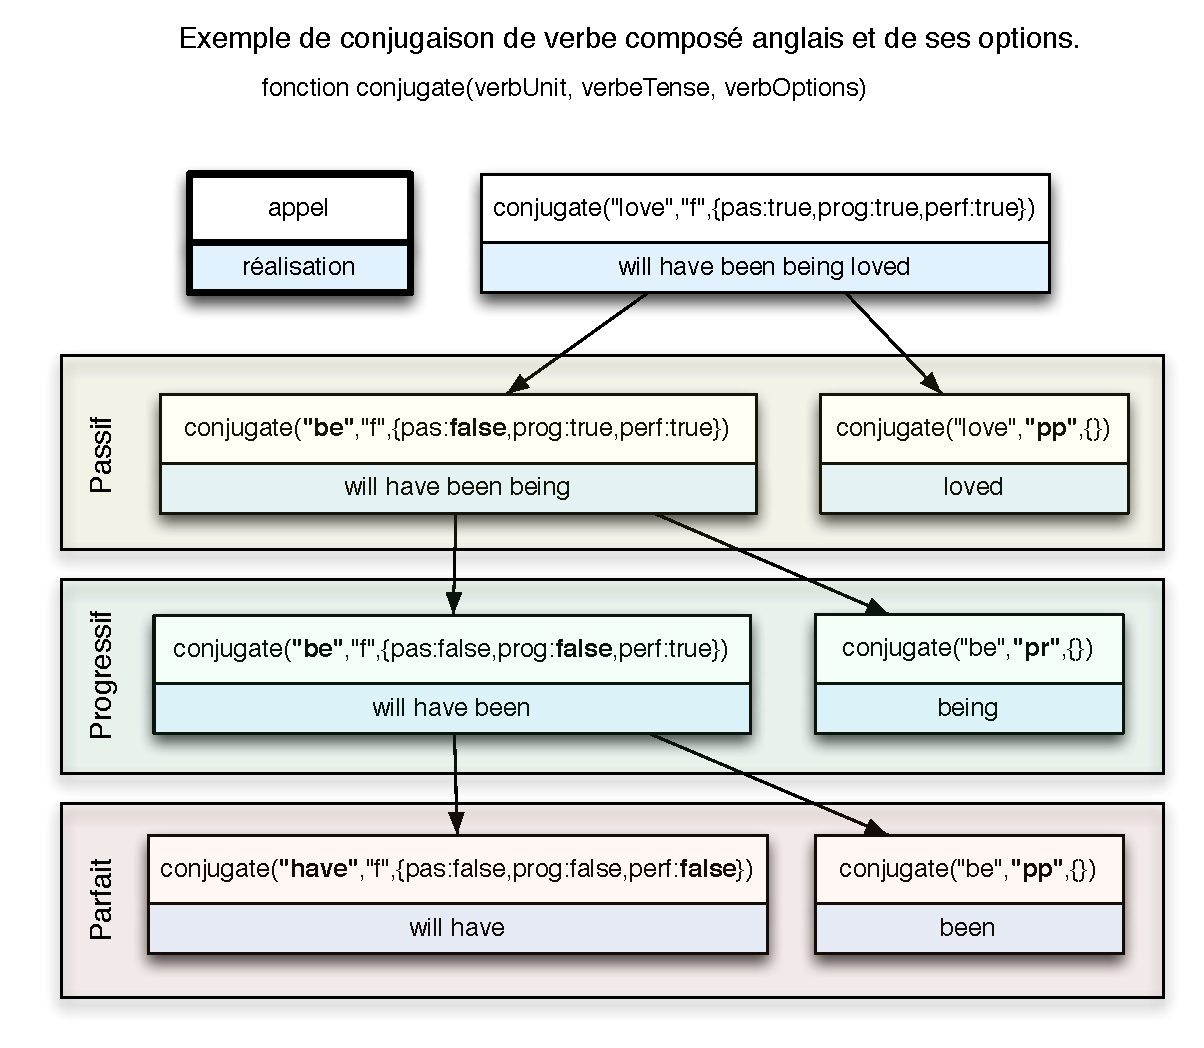
\includegraphics[scale=0.7]{love-conjOptions}
\label{figvOptEn}
\end{figure}

{\small{} Dans le schéma ci-haut, l'appel initial se trouve au sommet de l'arbre. Les 
cases enfants représentent les appels réscursifs qui sont appelés par le programme.
Si on observe les options de verbe, elles sont les trois \emph{true} initialement. Lors de
chaque appel récursif, on observe que les appels de gauche ont une option consommée(qui est devenue
\emph{false} par rapport à leur parent. Les trois options sont consommées dans l'ordre précisé plus tôt. 
Le verbe prescrit par l'option est appliqué à l'auxiliaire(gauche), alors que le participe obtient le verbe 
principal. Le temps de l'auxiliaire reste celui du verbe principal alors que le temps du participe est déterminé
 par l'option consommée. Au final, la récursivité se termine lorsqu'il n'y a pas d'option à consommer, donc en
présence d'un temps simple (present, past ou future). Il reste qu'à remonter l'arbre et à concaténer les résultats
pour obtenir le verbe désiré.}

\subsection{Syntagme adjectival}
\subsubsection{Positionnement de l'adjectif en français}
\paragraph{Anglais} Le positionnement de l'adjectif est toujours avant le nom. 
Aucune modification à \JSB{} n'a été apportée de ce côté-là.
\paragraph{Français}
Le positionnement de l'adjectif se fait majoritairement
après le nom. Par contre, avec plusieurs adjectifs communs, le placement
se fait avant. Une première approche à ce problème a été de créer
une fonction qui compterait les syllabes des adjectifs pour en déterminer
la position, car des adjectifs monosyllabiques se placent habituellement
avant le nom, comme \emph{long, court, gros ou vrai.} Par contre,
cette approche n'était pas prometteuse, car plusieurs adjectifs ayant
plusieurs syllabes se placent avant, comme \emph{premier}, et d'autres
courts se placent après, notamment les adjectifs de couleur. Une solution,
moins systématique, mais fonctionnant beaucoup mieux a été de dresser
une liste des adjectifs à placer avant le nom. Ensuite, un attribut
\emph{'pre'} a été manuellement ajouté à ces mots dans le fichier
\emph{dmf-lex.txt }utilisé pour générer le lexique. Lesdits adjectifs
ont donc eu un nouvel attribut dans le lexique français de \JSB{}.
Ensuite, en ajoutant l'option \emph{pos} à placer sur un adjectif,
l'utilisateur peut modifier la position de l'adjectif à l'intérieur
même du syntagme nominal associé. Si aucune option n'a été dictée
par l'utilisateur, le programme choisira comme option par défaut de
mettre l'adjectif après, à moins que celui-ci soit annoté comme étant
un adjectif antéposé dans le lexique. 


\subsection{Syntagme propositionnel}
\label{syntProp}

\subsubsection{Utilisation}

Le syntagme propositionnel est utilisé pour exprimer une proposition
relative. Dans \JSB{}, les syntagmes propositionnels sont appelés
à l'intérieur même d'un syntagme nominal lorsqu'ils sont complément
du nom ou à l'intérieur d'un syntagme verbal comme complément du verbe.
Voici quelques exemples d'utilisation du nouveau syntagme et comment
il s'inclut dans la structure syntaxique \JSB{}.

\begin{example}
\caption{Utilisation du syntagme propositonnel en français}
\begin{tabular}{p{7cm} | p{7cm}}
\hline 
\textbf{Français} \\
\hline
\begin{alltt}
1.S(NP(D("le"),
       N("maison").n("p"),
       SP(Pro("que"),
          Pro("je").pe(1).n("p"),
          VP(V("rencontrer").t("pc")))))
\end{alltt} &
\begin{alltt}
2.S(NP(D("le"),
       N("gens").n("p"),
       SP(Pro("qui"),
          VP(V("danser")))))
\end{alltt} \\
\real{Les maisons \textbf{que nous avons rencontrées}.} & \real{Les gens \textbf{qui dansent}.} \\
\hline
\begin{alltt}
3.S(NP(D("le"),
       N("fleur"),
       SP(Pro("dont"),
          Pro("je").pe(2),
          VP(Pro("me").pe(1),
             V("parler").t('pq')))))
\end{alltt} &
\begin{alltt}
4.S(Pro("je").pe(1),
    VP(V("vouloir"),
       SP(Pro("que"),
          Pro('je').pe(2),
          VP(V('partir').t('s')))))
\end{alltt} \\
\real{La fleur \textbf{dont tu m'avais parlé}.} & \real{Je veux \textbf{que tu partes}.} \\
\end{tabular}
\end{example}
\begin{example}
\caption{Utilisation du syntagme propositonnel en anglais}
\begin{tabular}{p{7cm} | p{7cm}}
\hline
\textbf{Anglais} \\
\hline
\begin{alltt}
1.S(NP(D("the"),
       N("house").n("p"),
       SP(Adv("that"),
          Pro("I").pe(1).n("p"),
          VP(V("meet").t("ps")))))
\end{alltt} &
\begin{alltt}
2.S(NP(D("the"),
       N("people").n("p"),
       SP(Pro("who"),
          VP(V("dance").t("p")))))
\end{alltt} \\
\real{The house \textbf{that we met}.} & \real{The people \textbf{who dance}.} \\
\hline
\begin{alltt}
3.S(NP(D("the"),
       N("car"),
       SP(D("which"),
          Pro("I").pe(2),
          VP(V("buy").t("ps")))))
\end{alltt} \\
\real{The car \textbf{which you bought}.}
\end{tabular}
\label{propEx}
\end{example}

\subsubsection{Propagation}

Dans une structure \JSB{}, le syntagme propositionnel ressemble à
une structure de phrase, c'est-à-dire que la propagation entre les
éléments intérieurs du syntagme se fait essentiellement entre le groupe
sujet et le groupe verbal. Par exemple, dans les syntagmes prépositionnels
\emph{dont tu m'avais parlé }et \emph{that we wet}, le verbe s'accorde
avec le pronom qui le précède, tout comme dans une phrase. En fait,
la propagation entre ses éléments est identique à celle d'une phrase.
La propagation est plus intéressante au niveau du parent du syntagme
propositionnel. Dans le cas où le syntagme en question est complément
du nom, il sera alors enfant d'un syntagme nominal. Alors, plusieurs
cas de figure peuvent subvenir. 
\begin{enumerate}
\item (\emph{français)}Le mot introduisant la proposition est \textbf{\emph{que}},
alors le noyau du syntagme nominal est le complément d'objet direct
de la proposition qui devrait normalement contenir un verbe. \JSB{}
créera un nouvel objet avec les propriétés du noyau et les donnera
au syntagme prépositionnel enfant comme étant les informations sur
le complément d'objet direct. Ces informations seront utilisées pour
accorder le participe passé avec auxiliaire avoir, si c'est le cas.
\item (\emph{français/}anglais)Le mot introduisant la proposition est \textbf{\emph{qui/who}}.
Dans ce cas, la proposition introduit une action qui est effectuée
par le noyau du syntagme nominal. Dans ce cas, les propriétés du noyau
sont transmises au verbe de la même manière qu'habituellement entre
sujet et verbe, donc le syntagme propositionnel recevra les informations
de genre et de nombre du noyau.
\item (\emph{français/anglais})Le mot introduisant la proposition est autre
que les précédents cités (cas par défaut). Dans ce cas, il n'y a pas
de propagation entre le syntagme nominal et le syntagme propositionnel
enfant. 
\end{enumerate}
Il est aussi possible que le syntagme parent soit un syntagme verbal,
auquel cas il ne semble pas y avoir de propagation à faire, comme
dans le cas no.3 précédent.

\subsection{Syntagme adverbial, prépositionnel et coordonné}

Les syntagmes adverbial, prépositionnel et coordonné avaient bien
été implémentés jusqu'à maintenant. Au cours de mon stage, je n'ai
pas eu à effectuer de changement sur ces syntagmes.

\section{Les différents types de phrases}
\JSB{} est maintenant doté d'options permettant de donner un mode
spécifique à la phrase. Sans option, les phrases sont déclaratives,
mais il est maintenant possible de réaliser des phrases exclamatives
et plusieurs types de phrases interrogatives différentes. 

\subsection{Exclamative}

L'option de la phrase exclamative est une option simple qui s'applique
seulement sur un objet \emph{S}, une phrase. La phrase exclamative
ne change en rien la structure initiale de la phrase et n'ajoute que
la ponctuation exclamative, soit le point d'exclamation. Il est intéressant
de noter qu'en français, il est possible d'avoir une phrase à teneur
exclamative et interrogative à la fois, par exemple: \emph{Qu'est-ce
que tu fais?!} est une phrase acceptée en français. C'est pourquoi
pour spécifier le ou les types de phrases, on devra faire appel à
l'option comme un objet et non pas en un paramètre. Par exemple, pour
l'exemple précédent, on devra appeler la phrase avec l'option suivante:
\emph{.typ(\{exc:true,int:true\}) . }Cette façon de faire permet de
plus de préciser le type de forme interrogative voulue. Il en sera
discuté plus bas. À noter que la double ponctuation a dû être ajoutée
manuellement au lexique pour être acceptée comme ponctuation acceptable.
En anglais, un tel usage ne semble pas être acceptable selon \emph{Antidote},
donc si les deux options sont passées, la ponctuation n'est pas valide
et la phrase aura la valeur de ponctuation par défaut(le point).

\subsection{Interrogative}
\label{question}

La phrase interrogative est beaucoup plus complexe.
Tout d'abord, dans la fonction de mise en forme de la phrase, la
ponctuation ajoutée sera le point d'interrogation. Par contre, avant
d'en arriver là, la réalisation de la phrase devra passer par une
série de tests pour savoir si la structure de la phrase doit être
changée. Cela est dû au fait que plusieurs types de questions peuvent
être passés en paramètres. Les différents types disponibles sont démontrés 
dans le \autoref{interro}.
\begin{table}[h]
\caption{Utilisation de la phrase interrogative}
\begin{tabular}{|c|c|c|}
\hline 
Appel de l'option & Effet -\small{\real{Exemple}}\\
\hline 
\hline 
\texttt{.typ(\{int:'yon'\})} & Question de type général.\textbf{ Est-ce que} telle action est arrivée? \\
\texttt{.typ(\{int:true\})} & \small{\real{Est-ce que le chat mange la souris?}}\\
\hline
\multirow{2}{*}{\texttt{.typ(\{int:'wos'\})}} & Question par rapport au sujet(qui). \textbf{Qui} a fait l'action?\\
& \small{\real{Qui mange la souris?}}\\ \hline
\multirow{2}{*}{\texttt{.typ(\{int:'wod'\})}} & Question par rapport à l'objet direct. \textbf{Qui} a subi l'action?\\
& \small{\real{Qui est-ce que le chat mange?}}\\
\hline 
\multirow{2}{*}{\texttt{.typ(\{int:'woi'\})}} & Question par rapport à l'objet indirect. À \textbf{qui} a-t-on fait
l'action?\\
&\small{\real{À qui est-ce que le chat mange la souris?}}\\
\hline 
\multirow{2}{*}{\texttt{.typ(\{int:'wad'\})}} & Question par rapport à l'objet direct. \textbf{Quoi} a subi l'action?\\
&\small{\real{Qu'est-ce que le chat mange?}} \\ \hline 
\multirow{2}{*}{\texttt{.typ(\{int:'whe'\})}} & Question par rapport à l'endroit. \textbf{Où }s'est déroulé l'action?\\
& \small{\real{Où est-ce que le chat mange la souris?}} \\ \hline 
\multirow{2}{*}{\texttt{.typ(\{int:'how'\})}} & Question sur la manière. \textbf{Comment }s'est déroulée l'action?\\
& \small{\real{Comment est-ce que le chat mange la souris?}} \\ \hline 
\end{tabular}
\label{interro}
\end{table}
\\
Le passage à la forme interrogative se fait en deux temps. D'abord,
si la structure de la phrase a à être modifiée, elle le sera, et ensuite
on ajoutera un préfixe à la phrase en tant que telle, par exemple
\emph{est-ce que }ou \emph{where} par exemple.

\paragraph{Commun aux deux langues}

Dans tous les cas, le programme fera un test sur la valeur du paramètre
\texttt{int}. Dans plusieurs cas, la structure de la phrase sera modifiée.
Bien évidemment, on peut passer l'option d'avoir une phrase interrogative
à une phrase déjà bien formée. Par contre, cela implique que la réponse
à la question est possiblement à l'intérieur même de la phrase. Il
faudra donc effacer cette partie de la phrase pour que celle-ci ait
du sens par la suite. Par exemple, si on désire avoir une question
par rapport à l'objet direct(quoi), sur la phrase suivante: \emph{Le
chat a mangé la souris, }la question désirée est: \emph{Qu'est-ce
que le chat a mangé?} Donc, le programme \JSB{} devra donc cerner
la partie faisant office d'objet direct(la souris, dans l'exemple)
et la retirer de la question.Pour cela, il est très important que
la structure d'arbre ait été bien construite par l'utilisateur. C'est-à-dire
qu'on trouvera le sujet d'une phrase comme étant le premier syntagme
nominal ou le premier pronom de la phrase, on trouvera l'objet direct
comme étant le syntagme nominal enfant du syntagme verbal principal
et de manière similaire l'objet indirect comme étant le groupe prépositionnel
issu du syntagme verbal principal. Si l'arborescence n'a pas été construite
de la manière attendue, le programme ne réagira pas de la bonne façon
et c'est valable pour beaucoup d'autres options. Les options diffèrent
légèrement entre les deux langues.

\paragraph{Français}

Pour les différentes options, il y a quatre cas de figure différents.
La troisième colonne représente respectivement les préfixes qui seront
ajoutés par la suite selon le type d'option. Les préfixes sont tirés
d'une table de règle, démontrée dans le \autoref{interroOptions} 
\begin{table}[h]
\centering
\caption{Les différentes options de la phrase interrogative}
\begin{tabular}{|c|c|c|}
\hline 
Option interrogative & Retrait du constituant & Préfixe\\
\hline 
\hline 
\texttt{true/yon} & Aucun & \real{"Est-ce que"}\\
\hline 
\texttt{wos} & Sujet & \real{"Qui est-ce qui"}\\
\hline 
\texttt{wod} & Objet direct & \real{"Qu'est-ce que"}\\
\hline 
\texttt{wad} & Objet direct & \real{"Qui est-ce que"}\\
\hline 
\texttt{woi} & Objet indirect & \real{"À qui est-ce que"}\\
\hline 
\texttt{whe} & Aucun & \real{"Où"}\\
\hline 
\texttt{how} & Aucun & \real{"Comment"}\\
\hline 
\end{tabular}
\label{interroOptions}
\end{table}


\paragraph{Anglais}

En anglais, le retrait des constituants ce fait de manière similaire,
par contre c'est un peu plus complexe, car on doit parfois rajouter
l'auxiliaire \emph{do, }qui doit s'accorder en fonction du sujet,
ce qui n'était pas le cas avec les préfixes français.\emph{ }Par exemple,
\emph{the dog runs} deviendra \emph{does the dog run?, }donc on doit
ajouter l'auxiliaire \emph{do }et faire en sorte d'avoir le verbe
à l'infinitif par la suite. Si le verbe appelé est au passé, alors
l'auxiliaire \emph{do }sera accordé au passé(\emph{did}) et si le
temps de verbe est le futur, l'auxiliaire sera \emph{will }au lieu
de \emph{do}. En anglais, les différentes options sont listées dans 
le \autoref{interroOptionsEn}.

\begin{table}[h]
\centering
\caption{Les différentes options de la phrase interrogative}
\begin{tabular}{|c|c|c|}
\hline 
Option interrogative & Retrait du constituant & Préfixe\tabularnewline
\hline 
\hline 
\texttt{true/yon} & Aucun & \real{"Do/will"}(accordé)\\
\hline 
\texttt{wos} & Sujet & \real{"Who"}\\
\hline 
\texttt{wod} & Objet direct & \real{"Who"}+\real{"do/will"}(accordé)\\
\hline 
\texttt{wad} & Objet direct & \real{"What"}+\real{"do/will"}(accordé)\\
\hline 
\texttt{woi} & Objet indirect & \real{"To who"}+\real{"do/will"}(accordé)\\
\hline 
\texttt{whe} & Aucun & \real{"Where"}+\real{"do/will"}(accordé)\\
\hline 
\texttt{how} & Aucun & \real{"How"}+\real{"do/will"}(accordé)\\
\hline 
\end{tabular}
\label{interroOptionsEn}
\end{table}

\section{Autres modifications}
\subsection{Liaison par le trait d'union}
Parfois, la mise en forme de
la phrase nécessite des traits d'union entre certains mots. C'est
plus fréquent en français, majoritairement lorsque le sujet et le
verbe sont inversés.  Les inversions sont utiles pour plusieurs phrases
interrogatives, mais l'approche utilisée et décrite à la \autoref{question}
 permet de former des questions sans inversion du sujet
et du verbe. Il y a aussi des cas où on pronominalisera le complément
d'objet direct avec un verbe impératif, par exemple: \emph{Mange-la!,
Retrouve-moi là-bas. }Dans ces cas précis, \JSB{} ne fait pas encore
la liaison et l'inversion, mais il est possible de le faire manuellement
avec une option \texttt{.lier()}, disponible avec tous les mots. En
appelant cette option, l'élément qui appellera la méthode \texttt{lier}
sera connecté avec le prochain mot par un trait d'union. C'est un
ajout simple à \JSB{} qui comble un manque en français, mais qui
permet aussi de créer des liaisons dans certains mots anglais aussi
qui le nécessite, notamment: \emph{well-known} ou \emph{blue-green}. L'\autoref{liaison}
présente l'utilisation de la liaison dans deux contextes.
\begin{example}
\centering
\caption{Utilisation de la liaison forcée}
\begin{tabular}{p{7cm} p{7cm}} 
\begin{alltt}
VP(V("rejoindre").t("ip").lier(),
   Pro("moi").pe(1),
   Adv("là-bas"))
\end{alltt} &
\begin{alltt}
NP(D("a"),
   A("blue").lier(),
   A("green"),
   N("algea"))
\end{alltt} \\
\real{rejoins-moi là-bas} & \real{a blue-green algea}\\
\end{tabular}
\label{liaison}
\end{example}


\subsection{Clone et déréférencement}
\label{clone}
\JSB{} a été spécialement développé pour fonctionner aisément avec
le web notamment par le fait qu'il est écrit en Javascript et qu'il
y a des options pour intégrer des balises HTML aux réalisations directement.
Il est donc normal de vouloir utiliser du code Javascript pour simplifier
la création d'objets \JSB{}. Par exemple, dans la phrase \emph{Les
pommes, je les ai cueillies. }il faudrait appeler la phrase avec cet
appel:
\begin{example}
\caption{}
\begin{alltt}
S(NP(D("le"),
     N("pomme").n("p")).a(","),
  Pro("je").pe(1),
  VP(V("cueillir").t("pc"),
     NP(D("le"),
        N("pomme").n("p")).pro()))
\end{alltt}
\real{Les pommes, je les ai cueillies.} 
\end{example}


Par contre, on appelle deux fois le même syntagme nominal. On pourrait
utiliser une variable Javascript pour éviter d'avoir à réécrire le
syntagme 2 fois, ainsi: \emph{var pom} = \texttt{NP(D("le"),N("pomme").n("p"))}. Par contre, l'appel de la phrase précédente en remplaçant par la
nouvelle variable ne donnera pas le résultat voulu. C'est-à-dire que
si nous appelons : 
\begin{example}
\caption{}
\begin{alltt}
S(pom,
  Pro("je").pe(1),
  VP(V("cueillir").t("pc"),
     pom.pro()))
\end{alltt}
\real{Elles, je les ai cueillies.}
\end{example}
\\


Malheureusement lors des deux appels de \textbf{pom}, les deux réalisations
seront similaires, car les deux méthodes pointent vers le même objet.
Lorsque le deuxième appel utilise la méthode \texttt{.pro()}, le syntagme
obtientla propriété de pronominalisation, donc les deux appels de
\textbf{pom} seront pronominalisés. Ce n'est pas le but désiré ici,
donc \JSB{} a maintenant une option pour créer un clone d'un objet
\JSB{}. Le clone hérite des propriétés initiales de l'objet, notamment
son genre, son nombre, sa personne, etc. Par contre, à partir du moment
où il est cloné, le nouvel objet ne partage plus ses propriétés avec
un autre appel du syntagme original. En bref: \\
\begin{table}
\caption{}
\begin{tabular}{|c|c|}
\hline 
\emph{var} \texttt{pom} = \texttt{NP(D("le"),N("pomme"))} & \real{la pomme}\\
\hline 
\hline 
\texttt{pom.clone.pro()} & \real{elle}\\
\hline 
\texttt{pom.clone.n("p")} & \real{les pommes}\\
\hline 
\texttt{pom} & \real{la pomme} {\small{}(sans influence des appels
précédents)}\\
\hline 
\end{tabular} 
\end{table}

\subsection{Élision}

\JSB{} a un module d'élision assez simple qui fonctionnait dans la plupart des cas de figure.
En plus de cela, quelques modifications simples ont été ajoutées.
\paragraph{Français}
L'élision fonctionnait bien, sauf pour le pronom/déterminant \emph{ce}. Celui-ci doit
s'élider lorsqu'il est devant le pronom \emph{en} ou devant une forme simple ou composée
du verbe \emph{être} commençant par une voyelle. Lorsque le module d'élision est appelé, la structure \JSB{} n'est plus 
et les constituants de la phrase ont déjà été convertis en \emph{string}. Cela fait en sorte
qu'il n'est pas possible de vérifier directement la classe du mot, ni sa forme de base pour savoir
si celle-ci est \emph{en} ou \emph{être}. 

Pour contrer cela, une table contenant le pronom \emph{en}
et les formes du verbe \emph{être} commençant par une voyelle a été ajouté aux ressources.
Lorsque le mot à élider est \emph{ce} et que le \emph{token} le précédant est présent
dans la table en question, \emph{ce} sera élidé en \emph{c'}. 

Autrement, \emph{ce} est
élidé en \emph{cet} devant un nom commençant par une voyelle. Finalement, dans les autres cas, 
il restera le même.

\paragraph{Anglais}
Devant un mot commençant par une voyelle, le déterminant \emph{a} devient \emph{an}.
La règle stricte spécifie que l'élision doit se faire si le mot suivante a sa première
syllabe qui sonne comme une voyelle. Donc, devant le mot \emph{unique} par exemple,
le \emph{a} devrait rester tel quel. \\
\begin{example}
\caption{}
\begin{tabular}{p{5cm} p{8cm}}
\begin{alltt}
NP(D("a"),
   A("unique"),
   N("scene"))
\end{alltt} &
\begin{alltt}
\end{alltt} \\
\real{*an unique scene} (\JSB{}) & \real{a unique scene}(correct)
\end{tabular}
\end{example}
\\
\\
Ce n'est pas le cas dans \JSB{}. Le programme aurait 
besoin de connaître la phonétique des syllabes pour être capable de discriminer
efficacement, ce qui n'est pas le cas. Tout de même, en majorité, lorsque le mot commence
par une voyelle, il devrait causer l'élision.

\section{Résultats}
Après toutes les modifications apportées à \JSB{}, on peut maintenant
dire que celui-ci est maintenant un réalisateur de texte français et anglais
prêt à l'emploi. Grâce aux maints ajouts au programme, la grande majorité
des phrases que l'on retrouve dans les textes de tous les jours peuvent
être correctement réalisées par \JSB{} de manière rapide. Pour ce
qui en est d'un ajout d'une troisième langue au programme, par l'ajout
du lexique et des tables de règles, on obtiendrait rapidement la plupart
des fonctionnalités de \JSB{}. Par contre, si la langue est quelque
peu différente au français ou à l'anglais pour ce qui est des accords,
il faudrait apporter directement des modifications au programme. À
noter aussi que le module de conjugaison est assez différent entre
les deux langues, donc il est à prévoir des modifications de ce côté
pour l'intégration d'une nouvelle langue, ainsi que dans la modification
vers la forme interrogative, qui est implémentée de manière similaire,
mais séparément dans le code, à cause de plusieurs différences notables.
La plupart des autres fonctionnalités sont adaptables facilement à
une autre langue future et ne requerront que peu ou pas de changements.
\section{Limitations et travail futur}
Il reste tout de même plusieurs fonctionnalités qui n'ont pas été
implémentées dans \JSB{}, soit parce que leur utilisation est moindre,
ou que l'implémentation semblait complexe. On y retrouve:

\begin{itemize}
\item Le passage automatique de \emph{he/she} vers \emph{it} en anglais
lors de la pronominalisation d'un objet ou d'un animal.
\item La dénombrement: \emph{the milk, }au lieu de \emph{a milk. De l'eau},
au lieu de \emph{une eau. }Aussi lié à l'utilisation de \emph{how much
vs how many }en anglais.
\item L'inversion sujet-verbe: \emph{Le garçon a aimé le jeu. $\rightarrow$ A-t-il
aimé le jeu?}
\item L'utilisation de la pronominalisation ainsi que de la négation, en
même temps: \emph{Je n'ai pas aimé le jeu $\rightarrow$ Je ne l'ai pas aimé.
}En ce moment, \emph{n'ai pas aimé} est la réalisation directe du
verbe. Par la pronominalisation, on ajoute le pronom avant, alors
qu'on devrait l'insérer quelque part à l'intérieur même de cette réalisation.
\item La contraction en anglais: \emph{do not $\rightarrow$ don't , I am $\rightarrow$ I'm , etc.}
\item L'élision de \emph{a} vers \emph{an} dans les cas où la première syllabe sonne comme une voyelle,
mais ne commence pas par une voyelle. Aussi dans le cas où ce n'est pas une voyelle, mais que la syllabe
sonne comme une voyelle.
\item La phrase interrogative avec \emph{combien}
\end{itemize}

\section{Conclusion}
\JSB{} est désormais un réalisateur de texte qui réalise bien plus
qu'il ne le faisait avant. L'apport fait a été une légère
modification au niveau du lexique(pour les adjectifs et les auxiliaires),
quelques ajouts au niveau des règles de chaque langue(participe, adverbes
interrogatifs et négatifs...) et plusieurs ajouts au niveau de \JSB{}
directement où un syntagme propositionnel a été ajouté, que le module
de conjugaison a été complètement changé, que la propagation a été
modifiée auprès de quelques syntagmes, etc. Pour s'assurer que le
tout fonctionne bien, des dizaines de tests unitaires ont été ajoutés pour assurer
la stabilité du programme lors d'ajouts futurs et les quelques démonstrations
qui existaient déjà de \JSB{} ont été mises à jour pour démontrer
les nouvelles fonctionnalités du programme.
\end{document}
